\documentclass[11pt,a4paper,final,notitlepage]{report}
\usepackage[utf8]{inputenc}
\usepackage{amsmath}
\usepackage{amsfonts}
\usepackage{amssymb}
\usepackage{fullpage}
\usepackage{graphicx}
\usepackage{grffile}
\usepackage{url}
\usepackage{enumitem}
\usepackage{xcolor}
\usepackage{textcomp}
\usepackage{listings}
\usepackage{varwidth}

\usepackage{caption}
\usepackage{subcaption}

\usepackage{stackengine,graphicx,trimclip,scalerel}

\renewcommand{\baselinestretch}{1.25} %Increase 

\makeatletter
\newcommand*{\toccontents}{\@starttoc{toc}}
\makeatother

\newcommand{\noNumberChapter}[2]{
    \setcounter{chapter}{#1}
    \setcounter{section}{0}
    \chapter*{#2}
    \addcontentsline{toc}{chapter}{#2}
}

\usepackage[nopar]{lipsum}
\usepackage{stackengine,graphicx,trimclip,scalerel}
\savestack\eye{\rotatebox{90}{$^\circ\mkern-6mu\raisebox{1pt}{)}$}}
\savestack\nose{\raisebox{3pt}{\scalebox{1}[-1]{\clipbox{0pt 1pt 0pt 0pt}{?}}}}
\savestack\mouth{\rotatebox{90}{(}}
\newcommand\Lenny{(\scalerel{\stackanchor[2pt]{\eye \nose \eye}{\mouth}}{)}}




\begin{document}

\title{ Major Project Report }

\author{ Tom Minor - Level H\\
 		 Major Project\\
 		 Bournemouth University, NCCA\\
 		 \\
 		 Supervised by Oleg Fryazinov, Adam Redford
		}

% Remove date
\date{}
\maketitle

\renewcommand{\abstractname}{Project Overview and Responsibilities}
%\\We have crazy integration, crazy asset production, crazy pipeline and our own GPU renderer - that's quite cool when you put it that way
\begin{abstract}

\begin{center}
\begin{varwidth}{\textwidth}
\begin{enumerate}
\item Fractal Renderer
\item FX
\item Pipeline\\
\end{enumerate}
\end{varwidth}
\end{center}

\textbf{CONTACT} is a near 3 minute long VFX sci-fi short, showing an astronaut’s state of mental decay after experiencing an encounter with a 5th dimensional being while in orbit. The team worked hard to create over 80 CG assets, 3 digital environments, and a bespoke fractal render engine for the evolving tunnel sequence at the height of the piece. Over 26 shots were composited into these built environments and costumes, fleshing out the narrative and blending together the live-action and the digital elements of the film.

\end{abstract}

\toccontents

\chapter{Introduction}

\begin{itemize}
	% Cite Odyssey?
	\item Created the initial pitch idea alongside Kyran Bishop, the result was his Space Odyssey inspired story that culminated in a dramatic psychedelic sequence, where my fractals were to be used. 
	\item I always planned to create some form of fractal lookdev tool, by joining a team of artists I made my overall job harder (the result absolutely has to look professional quality and needs to be finished or else the piece will suffer) but provided such a tool with some context.
	\item I took up additional roles as Pipeline TD and FX TD, given the large amount of work the team had to do it was unrealistic to expect myself to just work purely on the renderer.
	\item <Explain report overview>
\end{itemize}

\section{Goals}

\chapter{Initial Research}

\subsection{Fractal Sequence}
\subsection{FX Shots}

\section{Trying out existing stuff}
\subsection{Fractals in FX Software}
Looked at developing fractals in Houdini, may not need to develop a custom tool to visualise

Volumetric mandelbulb

Voxel Based

Slow to compute

\begin{center}
\includegraphics[scale=0.2]{"images/houdini_mandelbulb"}
\end{center}

Disney used houdini on BH6, but it's much too slow for our needs.

Need a custom tool

Houdini is still good for creature effects though, example noise shader goes here

Shadertoy has been a big deal in the past few years

GPU Accelerated rendering of implicit surfaces really efficient

Why not develop a custom tool just for fractal lookdev

\section{Reading the documentation and tutorials}











\chapter{Dynamics FX}

Had to create the effect of debris slowly drifting through space, so created the genesis of the destruction sequence as a base of the effect.

\section{Setting up the simulation}
\begin{itemize}
	\item Import the Voyager model as an FBX (with UVs) and convert the Maya hierarchy setup to Houdini groups
	\item Fracture a slightly pre-deformed version of the mesh, transfer the UVs and create new ones in the gaps
	\item Generate constraints between all nearby fractured pieces
	\item Manually paint on the strengths of each fractured piece, this is done by painting the strength onto the vertices and then finding the average strength of each fractured piece's vertices
	\item The core unit of voyager has a very high strength so it does not fall apart, as it has to be intact for the shot
	\item The manually painted strength values are multiplied by noise to get more variation
	\item The strength values are remapped using a curve for a less linear falloff
	\item Finally, transfer the strength values to the constraints and feed into the simulation
\end{itemize}

\section{Simulation Elements}
\begin{itemize}
	\item Fractured voyager with constraints
	\item Phantom collision geometry that initiates the destruction effect
	\item Zero gravity simulation, with torque and spin POP nodes to introduce interesting rotations into the simulation.
\end{itemize}

\section{Final Touches}
In the end, the simulation was exported to an alembic cache and Lewis processed it with a simple script that baked the animation data into locators. Using this method, we preserved animation ability for individual pieces if necessary but otherwise the simulation looked identical. Slowing down the simulation 20x in the Alembic's time scale was sufficient to give a convincing effect that the debris was slowly drifting, without completely stopping the simulation.






\chapter{Pipeline}

\begin{itemize}
	\item Dropbox isn't enough
	\item Need to version
	\item More effort at beginning of the project, having backups of every asset could save our asses in the end
	\item use perforce
	\item Other scripts can be added to the main pipeline suite
	\item Referencing pipeline required custom hooks that modify all referenced paths to be relative to \$CONTACTROOT, automated, idiot proof
	\item Referencing in 10 files and manually clicking student popup is tedious, on save and submit remove student/education flags
	\item Forces the team to think in a collaborative way, they literally cannot work on the same asset at the same time
	\item Took some getting used to, but now the artists are used to version control and it's benefits even if it's tedious at times
	\item Main development time spent on PySide Qt GUI stuff, after the initial time spent learning the P4 API and commands
	\item Technically cross application, the P4 and GUI side of things will work whereever pyside is available. Needs a few app specific tweaks such as file saving commands etc to work properly but wouldn't take long to port
	\item Various wizards to automate asset/shot/lookdev file structure generation because kyran made the layout super complex
	\item Allows us to analyse trends
	\item I setup Zync on Linux
\end{itemize}


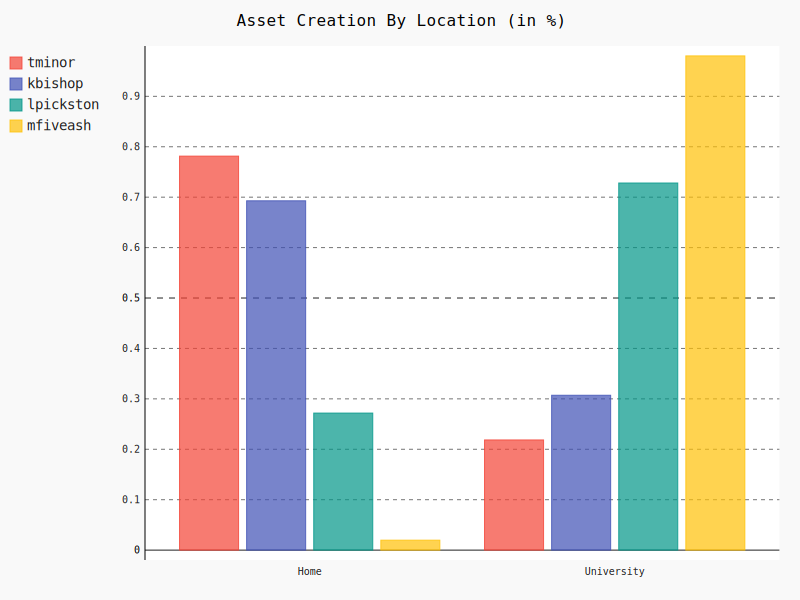
\includegraphics[width=\textwidth]{images/graph.png}





\chapter{Fractal Sequence}



\section{Fractal Tool Requirements}

\begin{itemize}
	\item How best to make this artist friendly (Nodegraph)
	\item What technique (ray marching)
	\item Use Optix because it's faster than what i can do
	\item Nodegraph needs runtime compilation, at least for geo
	\item Does require a little hacking to get runtime code generation
	\item Use NVRTC to compile code at runtime and plug into preexisting functions in the optix code
	\item Use hacky system commands to call nvcc directly if using CUDA 6.5 or less, aka, the uni systems
	\item Initial dev time for node graph, runtime compilation etc is long, but in theory will allow for rapid iteration once it works
	\item Everything is based on demo scene stuff, can use shadertoy as reference for loads of effects
	\section{Scene Management - Code Reflection}
		Need to change scene based on node graph
	\subsection{PTX Patching}
		\begin{itemize}
			\item Initial attempt, required research into the .ptx format
			\item Use NVCC to compile CUDA program into ptx code and patch into the Optix ptx code, then load into Optix
			\item Works on my machine and university workstations, but potentially undefined behaviour and not officially supported
			\item Relies on my own string handling functions
		\end{itemize}
	\subsection{Optix Callable Programs}
		\begin{itemize}
			\item Discovered this later in the project after reading the Optix documentation fully, initially didn't notice what it was because it's not used very often compared to the other aspects of optix and isn't really clear unless you know what it does.
			\item Use NVCC to compile CUDA program into ptx code and then tell Optix to use this as a 'callable program', basically replacing the ptx patching process with a well defined, built in functionality.
			
		\end{itemize}
\end{itemize}

\section{Rendering Strategy}
\begin{itemize}
	\item Render tiles
	\begin{itemize}
		\item For larger frame sizes this will give an opportunity for the calling program to return quickly and handle events
		\item Will use less GPU RAM, which is vital for HD frames on GPUs without lots of memory
		\item Has the potential to simplify implementation of other rendering algorithms in the future, for example Bidirectional Path Tracing stores light paths in an array that can become very large for huge images but is manageable for small tiles
	\end{itemize}

	\item Monitor the Optix rendering in a separate thread and copy over to host memory every half a second or so, this keeps the GUI responsive without over saturating the PCI-E bus (GPU -> CPU memory transfer) with constant memory copies.
	
\end{itemize}

\section{Output}
\begin{itemize}
	\item Save to EXR
	\item ZIP Compression, we need to render 650 1080p frames, a lot of data
	\item Multichannel
	\item Store each channel in a separate optix buffer
	\item Issue: Tedious to extend, but unlikely to be changed often
	
\end{itemize}

\subsection{Environment Camera}
\begin{itemize}
	\item Last minute request
	\item Required for relighting astronaut
	\item Optix makes this an easy thing to change, just fire rays in such a way that all possible directions are drawn at once like a fish eye lens.
	\item Thankfully the way I setup the various buffers maps directly onto the new camera model with no modification, adding the camera was as simple as defining a new ray generation program. This means that EXRs can be rendered with either the pinhole or environment camera and they will have identical data passes, this allowed us to use the exact same compositing networks to calculate the environment colour and have a 1:1 match for the relighting of the astronaut. Nuke and Maya accept the generated maps as environment maps with no issues.
\end{itemize}

\section{Colouring the fractal consistently}
\begin{itemize}
	\item Tried iteration count
	\item Tried comp only approaches
	\item Orbit traps are the way to go
	\item In the end we decided to use 3 different orbit traps encoded in the RGB channels of an EXR pass. This was configurable on a per scene basis if necessary (in the case of the tunnel scenes it was, the tube orbit trap gave useless values and needed manual tweaking)
\end{itemize}

\section{How the Shots were achieved}
\subsection{Side Sequence}

\begin{itemize}
	\item Use a mandelbulb, that slowly morphs from power 2 to power 5 as the sequence goes on. This
produces a growing effect.
	\item Apply a simple scene wide transformation that moves the mandelbulb slowly along the Z axis,
as well as rotates the fractal shape slowly around the Z axis.
	\item Set a low FOV of 30 to give the impression that the fractal shape is huge
\end{itemize}

\subsection{Tunnel Sequence}
The base shape was heavily inspired by the work of Syntopia's Shadertoy demos \cite{mengerjourney} \cite{kaljourney}.

\begin{figure}
\centering
\begin{subfigure}{.5\textwidth}
  \centering
  \includegraphics[width=.95\linewidth]{images/mengerjourney.png}
  \caption{Menger Journey \cite{mengerjourney}}
  \label{fig:sub1}
\end{subfigure}%
\begin{subfigure}{.5\textwidth}
  \centering
  \includegraphics[width=.95\linewidth]{images/kaljourney.png}
  \caption{Kaleidoscopic Journey \cite{kaljourney}}
  \label{fig:sub2}
\end{subfigure}
\caption{Two tunnel variations created by Syntopia, on Shadertoy}
\label{fig:test}
\end{figure}

\begin{itemize}
	\item The main tunnel shape was originally less organic, the shape I used as reference
\end{itemize}

\subsection{Reflected Visor Sequence}
This one was done last

\begin{itemize}
\item Power 5 mandelbulb constrained within a manually tweaked box shape (via intersection function)
to cut off the majority of it’s mass and keep it’s shape light and tendril like
\item This entire shape is then intersected with the tunnel shape, combining the organic shape of
the Mandelbulb with the hole in the tunnel. This creates an interesting silhouette.
\item Primarily used as a silhouette in the comp, so not many samples were required for usable
frames.
\item A high FOV of 110 is used to stretch out the shape even more and ease the process of mapping
it onto the visor.
\end{itemize}

\chapter{Future Improvements}

\begin{itemize}
	\item Look into methods besides distance estimation for more fractal possibilities, brute force approach
	\item Make the interface more artist friendly, with less reliance on understanding the maths
	\item Improve the input handling and allow for multiple input methods such as gamepads
	\item Some form of adaptive rendering to keep the viewport responsive
	\item Improve the light sampling algorithms using methods such as Bidirectional Path Tracing, VCM or Metropolis light transport.
	\item Provide a GUI interface for the lighting setup
	\item Move the batch rendering script's capabilities directly into the main renderer
	\item Screenspace CUDA shaders that make use of the various buffers available	
\end{itemize}


\chapter{Conclusion}

\part{In conclusion} I believe Romanesco is a useful and novel way of developing fractal objects in a visual effects context. The majority of currently available renderers are more of a novelty, designed to create nice images for a desktop background instead of a usable plate. Attempting to use existing renderers to create fractals is a plausible method, but suffers from poor interactivity due to long calculation times for the fractal structure.

Romanesco begins to fill in the gap between the currently available approaches, with more polish and focus put towards artist usability the more important issues such as fractals not behaving well enough for real world VFX shots can be minimised by the ease in which it is possible to iterate on the fractal design using the renderer.

Despite the final result being a fairly technical tool to use, the artistic feedback from the rest of the team has been vital in getting it to this stage. If I had decided to do this project solo, I don't believe it would have developed beyond the tech demo stage. By having a strong team surrounding me, especially in the compositing department, I saw first hand which features were actually important instead of focusing on the ones that I personally had an interest in. In the end, this is the reason we ended up with 600 frames worth of fractal sequence that was successfully used in integration with a live action piece.
%========================================================

\chapter{Renderer Implementation}

\begin{itemize}
	\item Overview
	\item Sphere tracing distance fields
	\item Path Tracing
	\item Progressive rendering
	\item Tile Based Rendering
	\item Modifying the scene at runtime using Reflection
\end{itemize}

\section{Performance}

\begin{itemize}
	\item Needs to be responsive, at least during the interactive preview
	\item Thought tile based rendering would help
	\item 
	\item rtContextSetTimeoutCallback
\end{itemize}


\section{Scene Management}

\subsection{Saving and loading scenes}
\begin{itemize}
	\item Not usable if scenes can't be saved
	\item Current implementation is more TD oriented, scenes are defined via CUDA functions that are compiled at runtime
	\item Camera information is encoded in comments at the top of the file
\end{itemize}

\subsection{Code Reflection}
Runtime compilation is necessary for allowing scene changes at runtime, specifically the ability to compile to .ptx code so it can be loaded into Optix as a callable function.
\subsubsection{Methods}

\begin{itemize}
	\item NVRTC - Available in CUDA 6.5 and up, faster and built in way of compiling.
	\item System NVCC - If using an older version of CUDA (such as on the university lab workstations), I try to use the system NVCC (hopefully available in path). This has the downsides of requiring the developer tools to be installed, as well as the performance overhead of launching and managing a subprocess. However, this allows me to render on a wider range of machines regardless of the performance impact.
\end{itemize}

\subsection{Runtime Patching}
Once the code is compiled, I needed some way to tell Optix to use it.

\begin{itemize}
	\item Manually patching the generated PTX code ( prone to error )
	\item Optix rtCallablePrograms ( officially supported way of doing it, found out later in the development process )
\end{itemize}

\subsection{Node Graph}

\begin{itemize}
	\item More artist friendly approach
	\item Spent a lot of time trying to develop this in the hope that it would aid the lookdev process
	\item Had to abandon the concept for the sake of getting the fractals lookdev'd on time
	\item Influenced the current design, which is basically a pure code version of what the node graph does
	\item An extra level of indirection, nodes -> CUDA code -> runtime patching
\end{itemize}

\subsubsection{Grammar Definition}
In order to properly write a parser, it was important to treat the node graph like a simple language. This was helpful in figuring out error conditions, for example if a domain operation is plugged into a distance operation \ref{fig:grammar}

\begin{figure}[h!]
	\includegraphics[scale=0.22]{nodegrammar}
	\caption{Grammar Definition}
	\label{fig:grammar}
\end{figure}

%========================================================


\nocite{*}

\bibliographystyle{plain-annote}
\bibliography{bib_icereport}
\end{document}
